\documentclass[12pt]{article}

\usepackage[utf8]{inputenc}
\usepackage[T1]{fontenc}
\usepackage[french]{babel}
\usepackage{amsmath, amssymb}
\usepackage{stmaryrd}
\usepackage{fancyhdr}
\usepackage{comment}
\usepackage{hyperref}
\usepackage{graphicx}
\usepackage{ebproof}

\newcommand{\defeq}{\ensuremath{\; \hat{=} \;}}
\newcommand{\FOL}{\ensuremath{\textup{\tiny{}FOL}}}
\newcommand{\FOML}{\ensuremath{\textup{\tiny{}FOML}}}
\newcommand{\false}{\textup{ff}}
\newcommand{\true}{\textup{tt}}
\newcommand{\M}{\ensuremath{\mathcal{M}}}
\newcommand{\I}{\ensuremath{\mathcal{I}}}


\usepackage{xcolor}
\newcommand{\raph}[1]{\textcolor{red}{#1}}

\definecolor{myblue}{rgb}{0,0.5,0.8}
\newcommand{\mpar}[1]{\marginpar{\color{red}\footnotesize\raggedright#1}}
\newcommand{\bpar}[1]{\marginpar{\color{myblue}\footnotesize\raggedright#1}}
\addtolength{\marginparwidth}{1cm}
\long\def\stephan#1{{\color{myblue} #1}}
\newcommand{\TRUE}{\textsc{true}}
\newcommand{\FALSE}{\textsc{false}}

\newtheorem{prop}{Propriété}

\bibliographystyle{plain}
\pagestyle{fancy}
%\setlength{\parskip}{12pt}

\title{%
  Compte rendu de stage de L3\\
  \vspace{8pt}
  \large On-the-fly Abstractions of Formulas in Proofs
Mixing First-Order Reasoning and Temporal Logic}
\author{Raphaël Le Bihan}



\begin{document}

\fancyhead[LEO]{Compte rendu de stage}
\fancyhead[REO]{Raphaël Le Bihan}
\fancyfoot[CEO]{\thepage}

\maketitle

Ce stage est effectué au Loria (Nancy), et a lieu du 08/06/2020 au 17/07/2020.
L'étudiant concerné est Raphaël Le Bihan en L3 au département d'informatique de l'ENS Paris-Saclay pendant l'année 2019-2020, l'encadrant du stage est Stephan Merz (Inria).
Le professeur supervisant le stage est Philippe Schnoebelen.

\setcounter{tocdepth}{2}
\tableofcontents

\section{Introduction}

\subsection{Contexte}

TLA$^+$ est un langage de spécification utilisé pour la vérification de systèmes distribués \cite{lamport2002}.
% Il permet de décrire le comportement attendu d'un système par implémentations successives OSEF
Il permet de décrire le comportement attendu d'un système par des propriétés temporelles exprimées avec des formules logiques, et d'écrire des preuves formelles pour ces propriétés.
TLA$^+$ s'appuie sur la logique TLA (pour Temporal Logic of Actions), introduite en 1994 par Leslie Lamport \cite{lamport1994}.

TLA représente l'exécution d'un système comme une suite d'états, où un état est l'affectation d'une valeur aux différentes variables du système.
Elle doit donc permettre de construire des formules afin de raisonner temporellement sur ces états.
TLA est un cas particulier de logique modale du premier ordre (FOML pour First Order Modal Logic).
Elle est constituée de la logique du premier ordre à laquelle s'ajoutent deux opérateurs temporels : $\square$ indiquant qu'une propriété est toujours vérifiée, et $'$ un opérateur décrivant la valeur d'une expression lors de l'état suivant.
\textcolor{myblue}{TLA$^+$} autorise également la définition de nouveaux opérateurs $d(x_1, \cdots, x_n) \triangleq e$ où $e$ est une formule FOML.

TLA$^+$ est aujourd'hui distribué avec TLAPS \cite{TLAPSurl} (pour TLA$^+$ Proof System), un assistant de preuve permettant de vérifier la validité de propriétés exprimées avec TLA$^+$.
Pour vérifier une propriété avec TLAPS, un utilisateur doit écrire une preuve avec TLA$^+$, consistant en une suite d'étapes \bpar{qui génèrent des?} appelées obligations de preuve.
Chaque obligation de preuve contient une formule FOML à prouver, et les hypothèses à utiliser pour prouver cette formule.
Lors de la lecture de la preuve par TLAPS, chaque obligation de preuve est traitée par un prouveur automatique de logique classique du premier ordre (Isabelle, Zenon ou Z3) ou de logique temporelle (ls4).

% \bpar{L'abstraction permet d'utiliser des outils qui ne comprennent qu'une partie des opérateurs sur des formules FOML.}
Ces prouveurs automatiques utilisent des logiques ne comprenant qu'une partie de la FOML.
Par exemple l'opérateur $\square$ est défini en logique temporelle mais pas en logique du premier ordre.
Il est alors nécessaire de définir une méthode de traduction correcte de la FOML vers la logique du premier ordre (FOL pour First Order Logic) et la logique modale (ML pour Modal Logic). %\raph{différence TL et ML}
Étant donnée une formule FOML $\phi$, on souhaite traduire cette formule en une formule FOL $\phi_\FOL$ telle que si $\vDash_\FOL \phi_\FOL$, alors $\vDash_\FOML \phi$ ; le principe est le même pour la logique modale.

Une méthode syntaxique appelée \og{}coalescing\fg{} (\og{}abstraction\fg{} en français) présentée en 2014 \cite{ARQNL2014} consiste à générer de nouveaux prédicats à partir des opérateurs FOML rencontrés n'étant pas reconnus dans la logique FOL ou ML.
On illustre cette méthode avec l'exemple suivant : l'opérateur $\square$ n'appartient pas à la logique FOL.
Etant donné un prédicat $P$ la formule FOML
\[ \phi = \square P \Rightarrow \square P \]
est valide.
On remarque qu'ici on peut déduire la validité de $\phi$ même sans savoir comment interpréter $\square$.
On abstrait alors la formule $\phi$ en :
\[ \phi_\FOL = \fbox{$\square P$} \Rightarrow \fbox{$\square P$} \]
où \fbox{$\square P$} est un nouveau prédicat.
$\phi_\FOL$ est valide et peut être prouvée en utilisant un prouveur automatique de logique du premier ordre.
On en déduit alors la validité de $\phi$ par correction de l'abstraction effectuée.

L'article de 2014 \cite{ARQNL2014} définit l'abstraction de la FOML vers la FOL et la ML et montre sa correction.
Il traite également le cas plus complexe de l'abstraction vers la FOL en présence d'opérateurs définis, et montre la complétude de l'abstraction pour la vérification de propriétés de {\color{myblue} sûreté} et \bpar{vraiment? sûreté seulement?} de vivacité, correspondant à la grande majorité des propriétés composants les spécifications en pratique. \raph{Utile de parler de la complétude ?} \stephan{non, rien à dire}

\subsection{Objectifs du stage}

\subsubsection{Remplacement de sous-formule par un opérateur défini}

Afin de vérifier certaines obligations de preuve dans l'implémentation actuelle de TLAPS, il est parfois nécessaire de masquer explicitement des sous formules en les remplaçant par des opérateurs définis.
Sans cela la vérification de ces obligations de preuve échoue.
Pour illustrer ce phénomène on considère l'exemple suivant :
étant donnés une constante $z$ (appelée variable rigide) et un prédicat unaire $P$ dont l'interprétation peut varier au cours du temps (dit flexible, ceci sera introduit formellement dans la suite du compte rendu), on veut montrer que la formule
\[ \phi = (\forall x \; : \; \square P(x)) \Rightarrow \square P(z) \]
est valide.
On propose les deux preuves suivantes écrites avec TLA$^+$ et lues par TLAPS.
\begin{center}
  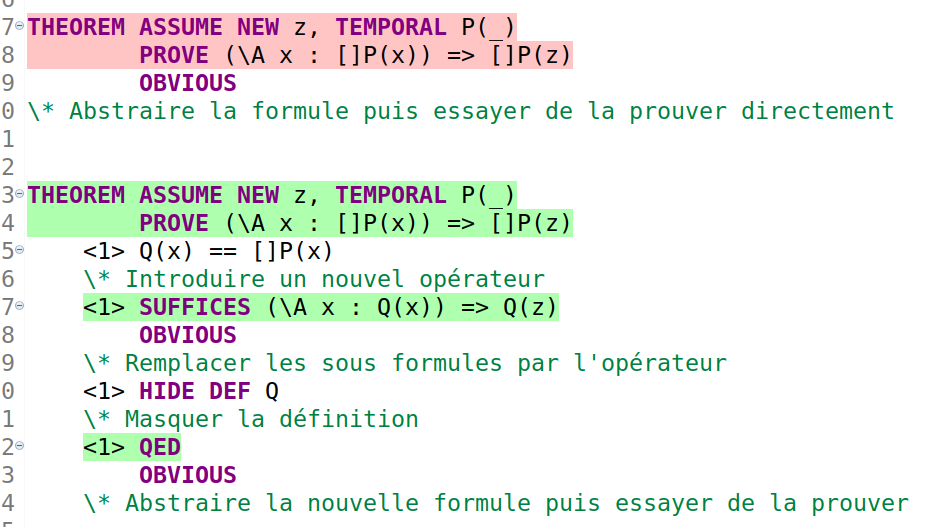
\includegraphics[width=0.8\linewidth]{tlaps_operateur}
\end{center}

La première preuve échoue car les sous formules $\square P(x)$ et $\square P(z)$ sont abstraits par des opérateurs différents, la formule FOL obtenue n'est donc plus valide.
La démarche utilisée dans la seconde preuve permet de vérifier la validité de $\phi$.

Un premier objectif sera d'étudier ce phénomène en confrontant ce résultat à la technique d'abstraction présentée l'article de 2014. On pourra chercher un moyen pour rendre possible de montrer $\phi$ sans avoir à introduire d'opérateur supplémentaire.

\subsubsection{Tautologies FOML non prouvables une fois abstraites en FOL}

Certaines formules FOML valides ne peuvent pas être prouvées en utilisant le processus d'abstraction.
On peut considérer l'exemple suivant :
étant donnée une formule $\phi$ FOML valide, \bpar{écrire $\Box\phi$ ici?} $\nabla \phi$ est également valide.
Pourtant la formule $\nabla \phi$ est abstraite en une formule FOL \fbox{$\lambda \vec{z} . \nabla \phi$}$(\vec{z})$ où $\vec{z}$ est un ensemble de variables.
La formule FOL obtenue n'étant pas valide, le processus d'abstraction défini dans l'article ne permet pas de déduire la validité de $\phi$.

Un deuxième objectif sera de chercher de nouvelles méthodes pour abstraire des formules FOML vers la FOL permettant de prouver d'avantage de tautologies FOML tout en gardant la correction.

\section{Activités pendant le stage}

Le stage a démarré le 08/06 et s'est terminé le 17/\textcolor{myblue}{07}, il a donc duré 6 semaines.
J'ai effectué pendant le stage les activités suivantes :
\begin{itemize}
\item
  Première semaine :
  j'ai lu l'article de 2014 sur le coalescing, lu et regardé des tutoriels et installé l'IDE pour travailler avec TLA$^+$ et TLAPS. J'ai fait quelques exercices pour m'entrainer à utiliser TLAPS ;
\item
  Deuxième semaine :
  j'ai fait quelques premiers tests avec TLAPS pour comprendre comment sont abstraites les formules dans l'implémentation actuelle.
  J'ai rédigé un fichier TLA$^+$ comparant les tautologies prouvables ou non en utilisant l'abstraction vers la FOL sans hypothèses supplémentaires.
  Le fichier contient également certaines idées pour modifier le processus d'abstraction afin de permettre de prouver plus de tautologies tout en conservant la correction.
  J'ai comparé les résultats du fichier avec les définitions données dans l'article.
\item
  Troisième et quatrième semaines :
  certaines tautologies ne sont pas prouvables une fois abstraites avec TLAPS, mais devraient l'être en utilisant les définitions dans l'article, il s'agit donc certainement d'une erreur d'implémentation.
  Plus généralement, il ne semble pas nécessaire d'après l'article d'utiliser des opérateurs pour masquer des sous formules comme présenté dans l'introduction.
  
  J'essaie de démontrer la propriété suivante : pour $\phi$ une formule FOML contenant des opérateurs définis, en notant $\widetilde{\phi}$ la même formule où on remplace les instances de l'opérateur par sa définition, si l'abstraction FOL de $\phi$ est une tautologie, alors l'abstraction FOL de $\widetilde{\phi}$ est également une tautologie.

  J'essaie pendant la troisième semaine de faire une preuve sémantique.
  Je veux montrer une propriété plus forte qui semble nécessaire pour utiliser l'hypotèse de récurrence.
  Je finis par trouver un contre-exemple à cette propriété.

  Je vois mal comment continuer, j'essaie pendant la quatrième semaine de faire une preuve syntaxique en utilisant la déduction naturelle.
  La plupart des cas de la récurrence sont triviaux sauf un.
  J'essaie d'utiliser un lemme, dont la preuve par récurrence est compliquée à cause de la définition de l'abstraction d'un opérateur défini posée dans l'article.
  Je propose une nouvelle définition, qui préserve la correction de l'abstraction.
\item
  Cinquième semaine :
  je commence la rédaction du compte rendu de stage.
\end{itemize}


\section{Définitions}

On présente ici les définitions utilisées dans la suite du compte rendu.

\subsection{Formules (ou expressions)}

\bpar{commenter l'amalgame entre termes et formules?}
On reprend les définitions données dans l'article de 2014.

\bpar{utiliser les environnements «théorèmes» de \LaTeX?}
\paragraph{Définition : formules FOML}
Etant donné un ensemble $\mathcal{O}$ d'opérateurs munis d'une arité, on définit une formule FOML récursivement
\[ e ::= \; x \; | \; v \; | \; op(\vec{e}) \; | \; e = e
  \; | \; e \Rightarrow e \; | \; \FALSE \; | \; \forall x : e \; | \; \nabla e \]
pour $op \in \mathcal{O}$, $x \in \mathcal{X}$, $v \in \mathcal{V}$ où $\mathcal{X}$ est l'ensemble des variables \emph{rigides}, $\mathcal{V}$ l'ensemble des variables \emph{flexibles}. $\mathcal{X}$ et $\mathcal{V}$ sont supposés infinis dénombrables et disjoints.
On n'autorise ici la quantification que sur les variables rigides.

Avec cette définition les opérateurs de $\mathcal{O}$ servent à définir à la fois les prédicats et les symboles de fonction de la logique du premier ordre.


\paragraph{Définition : formules FOL et ML}
On définit ensuite les formules FOL et ML.
Les formules FOL sont des formules FOML ne contenant pas de variable flexible ni de sous-formule $\nabla e$.
Les formules ML sont des formules FOML ne contenant pas de variable rigide, quantificateur, opérateur dans $\mathcal{O}$ ou égalité.

\subsection{Sémantique}

\raph{A voir si c'est vraiment utile (il me semble que oui sinon on ne sait pas ce qu'est une formule FOML valide).
  Ici dans la première preuve on ne considère que des modèles FOL, et dans la deuxième preuve on utilise seulement la déduction naturelle.}

La définition est légèrement différente de celle de l'article. \raph{A préciser ?}
\stephan{plutôt non}

\paragraph{Définition : structure de Kripke pour la FOML}
On définit une structure de Kripke pour la FOML $\M = (\I, \xi, \mathcal{W}, R, \zeta)$ où :
\begin{itemize}
\item
  $\I$ est une structure FOL usuelle, constituée d'un domaine $|\I|$ non vide et d'une interprétation des différents opérateurs de $\mathcal{O}$ comme des fonctions sur ce domaine ayant les arités correspondantes.
  On suppose de plus ici que le domaine contient deux éléments distincts $\false$ et $\true$.
\item
  $\xi$ est une valuation des variables rigides vers $|\I|$.
\item
  $\mathcal{W}$ est un ensemble non vide d'états, et $R \subseteq \mathcal{W} \times \mathcal{W}$.
\item
  $\zeta : \mathcal{V} \times \mathcal{W} \to |\I|$ est une valuation des variables flexibles.
\end{itemize}

\medskip

On définit ensuite l'interprétation d'une formule dans une structure par récurrence sur la formule.

\begin{itemize}
\item
  $\llbracket x \rrbracket_{\M, w} = \xi(x)$ et $\llbracket v \rrbracket_{\M, w} = \zeta(v, w)$ pour $x \in \mathcal{X}$ et $v \in \mathcal{V}$
\item
  $\llbracket op(\vec{e}) \rrbracket_{\M, w} = \I(op)(\vec{\llbracket e \rrbracket_{\M, w}})$
\item
  $\llbracket e_1 = e_2 \rrbracket_{\M, w} = \left \{
\begin{array}{l l}
  \true & \textup{ si } \llbracket e_1 \rrbracket_{\M, w} = \llbracket e_2 \rrbracket_{\M, w} \\
  \false & \textup{ sinon }
\end{array} \right .$
\item
  $\llbracket e_1 \Rightarrow e_2 \rrbracket_{\M, w} = \left \{
\begin{array}{l l}
  \true & \textup{ si } \llbracket e_1 \rrbracket_{\M, w} \neq \true \textup{ ou }
          \llbracket e_2 \rrbracket_{\M, w} = \true \\
  \false & \textup{ sinon }
\end{array} \right .$
\item
  $\llbracket \FALSE \rrbracket_{\M, w} = \false$
\item
  $\llbracket \forall x : e \rrbracket_{\M, w} = \left \{
\begin{array}{l l}
  \true & \textup{ si } \llbracket e \rrbracket_{\M[x \mapsto a], w} = \true \textup{ pour \textcolor{myblue}{tout} } a \in |\I| \\
  \false & \textup{ sinon }
\end{array} \right .$\\
en notant $\M[x \mapsto a]$ la structure correspondant à $\M$ où l'élément $a$ est affecté à la variable $x$.
\item
  $\llbracket \nabla e \rrbracket_{\M, w} = \left \{
\begin{array}{l l}
  \true & \textup{ si } \llbracket e \rrbracket_{\M, w'} = \true \textup{ pour \textcolor{myblue}{tout $w'$ tel que} } (w, w') \in R \\
  \false & \textup{ sinon }
\end{array} \right .$
\end{itemize}

\subsection{Opérateurs définis}

Étant donné une définition d'opérateur : $d(\vec{x_i}) \triangleq e_d$ où $\vec{x_i}$ est un ensemble de variables rigides et $e_d$ est une expression FOML (ne contenant pas d'occurence de $d$), on ajoute dans la définition récursive d'une formule FOML l'expression $d(\vec{e})$.
On définit ensuite son interprétation dans une structure FOML par \bpar{discutable mais je trouve ça plus facile à lire} $\llbracket d(\vec{e_i}) \rrbracket_{\M, w} = \llbracket e_d(\textcolor{myblue}{\vec{e}_i/\vec{x}_i}) \rrbracket_{\M, w}$.

\subsection{Expressions flexibles et rigides, positions Leibniz}

\bpar{Cette abstraction est définie seulement dans la section suivante.}
On définit récursivement l'abstraction d'une formule FOML $e$ vers la FOL en introduisant de nouveaux opérateurs.
Pour cela on définit d'abord les notions d'expression rigide et flexible et de position Leibniz.

\paragraph{Définition : Expression FOML rigide, flexible}
Une expression FOML $e$ est dite rigide ssi elle ne contient pas de variable flexible ou sous-expression $\nabla e'$.
Sinon elle est dite flexible.

\raph{Expliquer l'utilité des positions Leibniz ?} \stephan{oui}

\paragraph{Définition : Position Leibniz}
Une position est un emplacement pour un argument d'un opérateur défini.
Dans la définition $d(\vec{x_i}) \triangleq e_d$, la position correspondant à une variable $x_i$ est dite Leibniz ssi cette variable n'apparait pas dans une sous expression \bpar{j'éviterais d'utiliser $'$ car c'est un opérateur en TLA, aussi $e$ n'est pas utilisé ici} $\nabla e'$.


\subsection{Abstraction vers la FOL}

La définition suivante pour l'abstraction d'un opérateur défini est différente de celle posée dans l'article\stephan{~\cite{ARQNL2014}}.
Ici les positions non Leibniz sont retirées à l'opérateur FOL, alors qu'elle sont laissées dans l'article de la FOL.
\raph{Utile de le préciser ?} \stephan{Peut-être donner un exemple après la définition?}
Les propriétés de correction de l'abstraction données dans l'article sont préservées avec cette nouvelle définition, en reprenant les mêmes preuves qu'il suffit d'adapter pour le cas des opérateurs définis.

\paragraph{Définition : Abstraction vers la FOL}

On définit récursivement l'abstraction vers la FOL d'une formule FOML $\phi$.
% Pour $y$ une liste de variables rigides.
\raph{On pose ici directement comme définition que l'abstraction d'un $\nabla e$ est \fbox{$\lambda z . \nabla e$} où $z$ est l'ensemble des variables libres rigides de $e$, pour ne pas s'encombrer avec la liste y.} \\
\begin{itemize}
\item
  $x_\FOL = x$ et $v_\FOL = v$ pour $x \in \mathcal{X}, v \in \mathcal{V}$. En FOL $v$ est alors considérée comme une variable rigide.
\item
  $op(\vec{e})_\FOL = op(\vec{e_\FOL})$ pour $op \in \mathcal{O}$
\item
  $(e_1 = e_2)_\FOL = ({e_1}_\FOL = {e_2}_\FOL)$
\item
  $(e_1 \Rightarrow e_2)_\FOL = ({e_1}_\FOL \Rightarrow {e_2}_\FOL)$
\item
  $\FALSE_\FOL = \FALSE$
\item
  $(\forall x : e)_\FOL = \forall x : e_\FOL$
\item
  \( (\nabla e)_\FOL = \fbox{$\lambda \vec{x_i} . \nabla e$}(\vec{x_i}) \) où $\vec{x_i}$ est \bpar{c'est donc une liste \dots} l'ensemble des variables rigides libres de $e$ ordonné arbitrairement.
  Ces opérateurs \stephan{lesquels?} sont identifiés modulo $\alpha$-équivalence.
\item
  \( d(\vec{e_i})_\FOL = \fbox{$d_{\vec{\epsilon_i}}$}(\vec{e_j}) \) où on note :
  \( \epsilon_i = \left \{
    \begin{array}{l l}
      e_i & \textup{ si $e_i$ est flexible } \\
      * & \textup{ sinon }
    \end{array} \right . \)\\
  et où les arguments $\vec{e_j}$ sont les expressions rigides parmi les $\vec{e_i}$ en conservant l'ordre des arguments
\end{itemize}


\subsection{Remplacement d'opérateur défini}

On se place dans le cas où les formules FOML ne peuvent contenir qu'un seul opérateur défini $d$, donné par sa définition $d(\vec{x_i}) \triangleq e_d$.
On définit pour $\phi$ une formule FOML la formule $\widetilde{\phi}$ correspondante, où on remplace chaque occurence de $d$ par la formule $e_d$ en effectuant des substitutions pour les arguments de $d$. Formellement :
\begin{itemize}
\item
  $\widetilde{x} = x$, $\widetilde{v} = v$ pour $x \in \mathcal{X}$, $v \in \mathcal{V}$
\item
  $\widetilde{op(\vec{x_i})} = op(\vec{\widetilde{x_i}})$ pour $op \in \mathcal{O}$
\item
  $\widetilde{(e_1 = e_2)} = (\widetilde{e_1} = \widetilde{e_2})$
\item
  $\widetilde{(e_1 \Rightarrow e_2)} = (\widetilde{e_1} \Rightarrow \widetilde{e_2})$
\item
  $\widetilde{\FALSE} = \FALSE$
\item
  $\widetilde{(\forall x : e)} = \forall : \widetilde{e}$
\item
  $\widetilde{\nabla e} = \nabla \widetilde{e}$
\item
  $\widetilde{d(\vec{e_i})} = e_d(\vec{\widetilde{e_i}/x_i})$
\end{itemize}


\section{Propriétés et preuves}

\bpar{éviter «du papier de 2014»}
\subsection{Propriétés du papier de 2014}

L'article\stephan{~\cite{ARQNL2014}} montre \bpar{énoncer les propriétés qui sont utiles par la suite?} différentes propriétés, en particulier la correction de l'abstraction de la FOML vers la FOL et la ML.
Les définitions utilisées ici étant différentes, on peut s'assurer que les propriétés énoncées dans l'article restent valides même avec ces définitions, en reprenant le même schéma de preuve que dans l'article.

\subsection{Remplacement de sous-formule par un opérateur défini}

Intuitivement remplacer une sous-formule FOML par un opérateur défini frais ne semble pas nécessaire pour démontrer une obligation de preuve en utilisant l'abstraction FOL.
On peut en effet comparer ce procédé à l'expansion d'une macro.

On reprend l'exemple présenté dans l'introduction.
L'obligation de preuve contient la formule en TLA$^+$ \bpar{dire que $z$ est rigide} $(\forall x : \square P(x)) \Rightarrow \square P(z)$ qui correspond en FOML à $(\forall x : \nabla P(x)) \Rightarrow \nabla P(z)$ où $P$ est un opérateur défini dont on ignore la définition.

On peut vérifier que le processus d'abstraction donne la formule FOL :
\( (\forall x : \fbox{$\lambda x . \nabla P(x)$}(x)) \Rightarrow \fbox{$\lambda z . \nabla P(z)$}(z) \)
qui est valide puisque les deux opérateurs sont $\alpha$-équivalents.
Que TLAPS ne permette pas de prouver automatiquement la formule en TLA$^+$ semble donc être une erreur d'implémentation.
On veut donc essayer de montrer la propriété suivante :

\begin{prop}
  \label{prop_sem}
Soit $d(\vec{x_i}) \triangleq e_d$ un opérateur défini, et $\phi$ une formule FOML pouvant contenir des occurences de $d$.
Si $\vDash_\FOL \phi_\FOL$ alors $\vDash_\FOL \widetilde{\phi}_\FOL$.
\end{prop}

\subsection{Tentatives de preuve pour la propriété}

\paragraph{Preuve sémantique}

J'ai d'abord essayé de faire une preuve sémantique par récurrence sur $\phi$.
Comme la FOML utilise les opérateurs à la fois comme symboles de fonction et prédicats de la logique du premier ordre usuelle, on aimerait montrer plus généralement que pour toute structure FOL $\M$, $\llbracket \phi_\FOL \rrbracket_\M = \llbracket \widetilde{\phi}_\FOL \rrbracket_\M$.
Plus précisément, comme les opérateurs générés lors des abstraction de $\phi$ et $\widetilde{\phi}$ sont différents, on veut montrer la propriété :
\begin{prop}
Soit $d(\vec{x_i}) \triangleq e_i$ un opérateur défini, et $\phi$ une formule FOML pouvant contenir des occurences de $d$.
%\bpar{Ici on a $\phi$, $\phi_{\FOL}$ et $\widetilde{\phi}_{\FOL}$, les deux dernières n'étant pas définies dans cette note \dots}
Soit $\mathcal{M}$ un modèle FOL où on peut interpréter $\widetilde{\phi}_\FOL$ (çàd un modèle dans lequel les opérateurs \framebox{$\lambda z . \nabla e$} générés lors de l'abstraction de $\widetilde{\phi}$ ont une interprétation).
On peut compléter $\M$ en un modèle FOL $\M_d$ où on peut interpréter $\phi_\FOL$ en ajoutant les interprétations suivantes pour les opérateurs \framebox{$\lambda z . \nabla e$} et \framebox{$d_{\vec{\epsilon}}$} générés lors de l'abstraction de $\phi$ :
\begin{enumerate}
\item
  Pour les opérateurs \framebox{$\lambda z . \nabla e$} ayant déjà une interprétation dans $\M$ (donc ayant déjà été générés lors de l'abstraction de $\widetilde{\phi}$) :
  \[ \I_d(\framebox{$\lambda z . \nabla e$}) = \I(\framebox{$\lambda z . \nabla e$}) \]
\item ... * une certaine définition pour les opérateurs générés lors de l'abstraction de $\phi$ *
\end{enumerate}
\end{prop}

La preuve de cette propriété par récurrence échoue car dans certains cas on doit recombiner des modèles, par exemple pour le cas $\phi = \phi_1 \Rightarrow \phi_2$ où on doit former $\M_d$ à partir des modèles $\M_{d1}$ et $\M_{d2}$ ce qui est impossible dans certains cas.

\paragraph{Preuve syntaxique}

J'ai ensuite essayé de faire une preuve syntaxique en utilisant la déduction naturelle.
Par correction et complétude, il suffit de montrer la propriété suivante :
\begin{prop}
  Pour toute formule FOML $\phi$ et tout ensemble de formules FOML $\Gamma$,
  si $\Gamma_\FOL \vdash \phi_\FOL$, alors $\widetilde{\Gamma}_\FOL \vdash \widetilde{\phi}_\FOL$.
\end{prop}
On montre cette propriété par récurrence sur la hauteur de la dérivation de $\Gamma_\FOL \vdash \phi_\FOL$.
La logique FOL étudiée ne contient pas les symboles $\land, \lor, \exists, \neg$, on étudie donc seulement les règles ax, RAA, $\Rightarrow_I$, $\Rightarrow_E$, $\forall_I$, $\forall_E$, $\bot_E$.
%On peut montrer les cas RAA, $\Rightarrow_I$, $\Rightarrow_E$, $\bot_E$ en appliquant les définitions et l'hypothèse de récurrence.
%Le cas ax ne pose pas de difficulté.
%On considère maintenant les cas $\forall_I$ et $\forall_E$.
La preuve par récurrence fonctionne sans difficulté particulière pour tous les cas sauf $\forall_I$ et $\forall_E$.
On parvient à montrer le cas $\forall_I$ :

\bigskip

On suppose qu'il existe une preuve de
\begin{prooftree}
  \hypo{ \Gamma_\FOL \vdash \psi }
  \infer1[$\forall_I$]
  { \Gamma_\FOL \vdash \phi_\FOL = \forall x : \psi }
\end{prooftree}, où $x \notin fv(\Gamma_\FOL)$.

Par analyse de cas sur la définition de $\phi_\FOL$ on trouve que $\phi = \forall x : \phi_1$ avec ${\phi_1}_\FOL = \psi$ :
\begin{prooftree}
  \hypo{ \Gamma_\FOL \vdash {\phi_1}_\FOL }
  \infer1[$\forall_I$]
  { \Gamma_\FOL \vdash \forall x : {\phi_1}_\FOL }
\end{prooftree}

On peut alors appliquer l'hypothèse de récurrence, il existe donc une dérivation de $\widetilde{\Gamma}_\FOL \vdash \widetilde{\phi_1}_\FOL$.

On peut montrer que si $x \notin fv(e_\FOL)$, alors $x \notin fv(\widetilde{e}_\FOL)$ par récurrence sur $e$. On en déduit que $x \notin fv(\widetilde{\Gamma}_\FOL)$.

On applique donc la règle $\forall_I$ pour obtenir la dérivation suivante :\\
\begin{prooftree}
  \hypo{ \widetilde{\Gamma}_\FOL \vdash \widetilde{\phi_1}_\FOL }
  \infer1[$\forall_I$]
  { \widetilde{\Gamma}_\FOL \vdash \forall x : \widetilde{\phi_1}_\FOL } 
\end{prooftree}
où $\forall x : \widetilde{\phi_1}_\FOL = \widetilde{(\forall x : \phi_1)}_\FOL = \widetilde{\phi}_\FOL$.

\bigskip \bigskip
  
Le cas $\forall_E$ pose problème car certaines formules FOL ne peuvent pas être formées en abstrayant des formules FOML.
On peut s'en convaincre avec l'exemple suivant : on considère $d$ un opérateur défini unaire et dont la position n'est pas Leibniz, et $v$ une variable flexible.
Abstraire la formule FOML $d(v)$ donne la formule FOL \( \fbox{$d_v$} \), car $v$ est flexible à un emplacement non Leibniz.
Alors la formule FOL \( \fbox{$d_*$}(v) \) ne peut pas être abstraite depuis la FOML.

\begin{comment}
\raph{En fait ici, la définition de l'abstraction utilisée dans le papier posait problème car on pouvait avoir des formules du type \fbox{$d_v$}$(x)$, ce qui n'est plus le cas maintenant (le prédicat abstrait \fbox{$d_v$} n'a pas d'argument)\\
  Les formules \fbox{$d_*$}$(v)$ ne posent pas de problème ici.}
\end{comment}
\begin{comment}
On ne peut donc pas appliquer l'hypothèse de récurrence dans le cas $\forall_E$ où :
\begin{prooftree}
  \hypo{ \Gamma_\FOL \vdash \forall x : \psi }
  \infer1[$\forall_E$]
  { \Gamma_\FOL \vdash \phi_\FOL = \psi\{x \mapsto t\} }
\end{prooftree}
car il n'existe pas a priori de
\end{comment}

\section{Conclusion}

J'ai passé la plupart du temps du stage à essayer de démontrer la proposition \ref{prop_sem}, je n'ai finalement pas réussi.
Les schémas de preuve produits ont néanmoins permis de révéler certaines différentes difficultés rencontrées, et certaines parties peuvent être réutilisées indépendemment du processus d'abstraction utilisé.
La plupart des difficultés rencontrées proviennent des interprétations \og{}imprévues\fg{} des opérateurs générés pendant l'abstraction.
Par exemple dans une dérivation en FOL utilisant la déduction naturelle, un séquent $\Gamma \vdash \phi$ pose problème si $\phi$ ou une formule de $\Gamma$ ne peut pas être formée en abstrayant une formule FOML.
Ces difficultés m'ont amené à essayer d'utiliser des définitions différentes de celles de l'article, qui sont celles présentées dans le compte rendu.
Il aurait sans doute été judicieux de passer plus de temps à réfléchir aux définitions utilisées et à leurs conséquences.
Ceci pourrait permettre de faciliter les preuves, et d'obtenir une méthode d'abstraction de la FOML vers la FOL permettant de prouver plus de tautologies FOML en utilisant la FOL.


\begin{comment}
\raph{%
TODO :
\begin{enumerate}
\item
  Confronter le CR et les documents de conseil des profs,
  \url{http://www.lsv.fr/~baelde/m1/reports.html}
  \url{http://www.lsv.fr/~leroux/To_be_downloaded/Teaching/Stages/conseils_informels_stage.pdf}
\item
  Rédiger + expliquer mes preuves
\item
  Envoyer le CR à Stephan + mes profs
\end{enumerate}
}
\end{comment}

\bibliography{biblio_cr}

\end{document}